We explore three different adaptation strategies for mesh adaptation based on the VMS-based estimated error. 

\subsection{Zonal Refinement/Adaptation}

The first strategy we employ is error estimator based zonal refinement/adaptation. 
In this strategy, we obtain an initial solution on a baseline mesh for the problem at hand. The VMS-based error estimator is then applied to the solution corresponding to this mesh, and based on the estimated error, the mesh is refined by a factor of 2 in particular zones where high error values are found. Estimated error for this adapted mesh is then calculated, and the mesh is again refined by a factor of 2 in zones of high error. This process is repeated till it is computationally feasible, or a convergence is reached.

This strategy is represented in Figure \ref{fig:zonal_based_strat}

\begin{figure}[H]
	\centering
	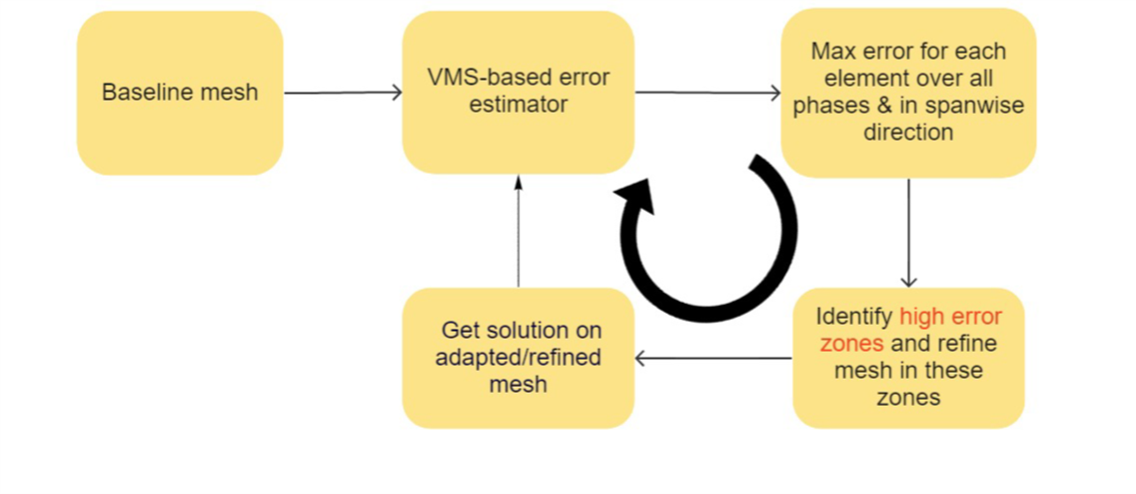
\includegraphics[width=1\textwidth]{figures/adapt_strat/zonal_based.png}
	\caption{Zonal Refinement/Adaptation Strategy}
	\label{fig:zonal_based_strat}
\end{figure}

\subsection{Nodal Size Field-based Adaptation}

The second strategy we employ is fully automated mesh adaptation based on the VMS-based error estimator. In this strategy, the estimated error and a specified target error are used to compute the desired mesh size or resolution in a local fashion, i.e., at every mesh vertex. We refer to this as the nodal size field, and the mesh is refined or coarsened based on this nodal size field. 

In this adaptive strategy, the VMS-based error is calculated on the initial mesh. Based on the estimated error, a nodal size field is calculated using the following equation \cite{zhang19}

\begin{equation}
	\frac{e_k}{\tilde{e}_k} = \left(\frac{h_{old}}{h_{new}}\right)^{m+N/2} 
	\label{eq:diez}
\end{equation}

Here, $e_k$ is the measured local error (in the $\HOne$-seminorm) at an element $k$, $\tilde{e}_k$ is the target error for an element specified by the user, $m$ is the polynomial order of the approximation space (i.e., $m=1$ for the linear finite elements used currently) , and $N$ is the number of spatial dimensions. $h_{old}$ is current size of the element, and $h_{new}$ is the desired new mesh size.
This new mesh size at the element level is assembled at the node/vertex level to perform mesh adaptation.
This strategy is represented in Figure \ref{fig:size_based_strat}.

\begin{figure}[H]
	\centering
	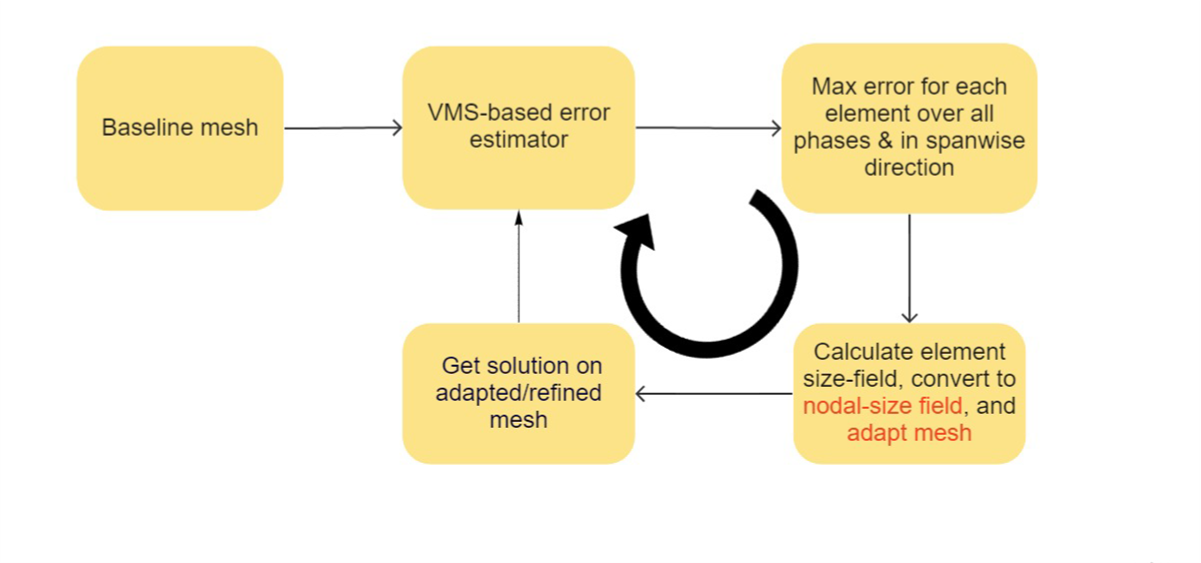
\includegraphics[width=1\textwidth]{figures/adapt_strat/size_based.png}
	\caption{Nodal Size Field-based Refinement/Adaptation Strategy}
	\label{fig:size_based_strat}
\end{figure}

\subsection{Feature-based Refinement/Adaptation}

The third strategy is to employ feature-based refinement/adaptation. This allows for refinement around dominant flow features and also along the path/trajectory of such features, for example, in the case of flow over surging airfoils, the paths of leading and trailing edge vortices (LEV and TEV) over a surging cycle using vortex tracking. By running an initial simulation, we can get information on the approximate path that a certain feature will follow, estimate the error along this path, and perform refinement/adaptation along this path.

This strategy is represented in Figure \ref{fig:feature_based_strat}.

\begin{figure}[H]
	\centering
	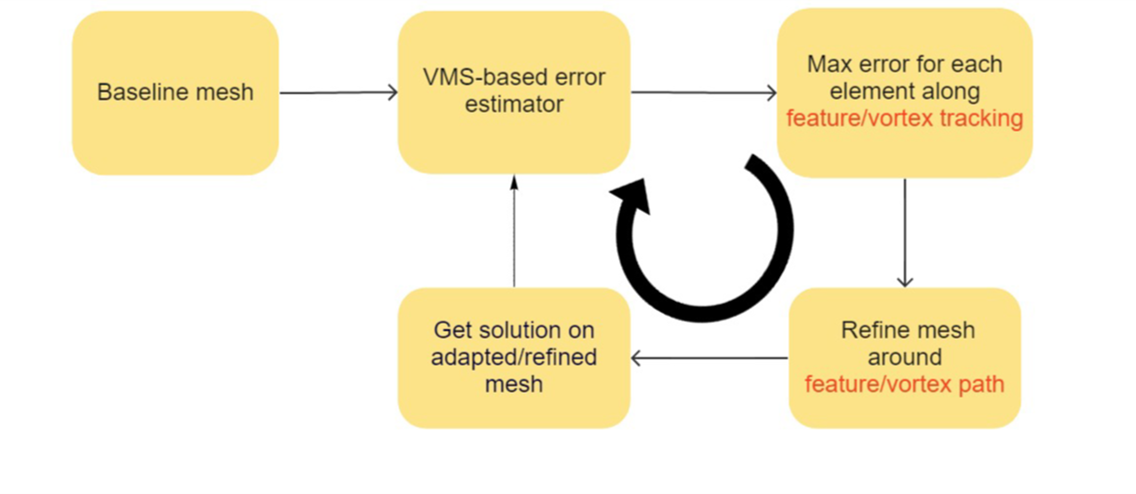
\includegraphics[width=1\textwidth]{figures/adapt_strat/feature_based.png}
	\caption{Feature-based Refinement/Adaptation Strategy}
	\label{fig:feature_based_strat}
\end{figure}

Further details and applications of these three strategies are included in Chapter \ref{chap:zonal_adapt_results}




